\chapter{Fundamentos de Sistemas Multiportadora}
\label{sec:fundamentos_dmt}

Os sistemas de comunicação multiportadora têm seu surgimento motivado pela necessidade de utilizar as características do canal de transmissão na modulação, visando aumentar a quantidade de informação que pode ser transmitida pelo sistema. A partir de 1948, com o desenvolvimento da teoria da informação, diversas tentativas do uso de sistemas multiportadoras foram executadas com este propósito. A de maior sucesso efetivou-se somente em 1993, quando a modulação denominada multitom discreto (DMT) foi padronizada para utilização na transmissão de dados através de linhas telefônicas, tecnologia conhecida como linha de assinante digital (DSL). No mesmo momento, também emergiu a modulação por divisão ortogonal de frequência (OFDM), atualmente amplamente utilizada em aplicações como radiodifusão sonora digital, televisão digital, redes sem fio de área local (WLAN) e quarta geração de telefonia móvel (4G).

A essência dos sistemas DMT e OFDM é dividir a largura de banda disponível para transmissão em vários subcanais, visando promover maior eficiência espectral (maior taxa de dados transmitidos por largura de banda do sistema) a partir das características individuais de cada subcanal. Para canais de transmissão seletivos em frequência ou com dispersão razoável, esta técnica garante ganhos significativos de desempenho em relação a sistemas de comunicação de portadora única. Por este motivo, os sistemas multiportadora apresentam-se como a escolha mais atrativa para oferecer serviços de altas taxas de dados em canais com interferência inter-simbólica significativa \cite{ee379c}.

Nesta seção, serão apresentados os conceitos fundamentais de sistemas OFDM e DMT, com enfoque para o último, já que este trabalho toma as redes DSL como cenário de aplicação das técnicas de mitigação de interferência desenvolvidas. Além disso, apresenta-se uma análise quantitativa e qualitativa dos fenômenos de interferências inter-portadora (ICI) e interferência inter-simbólica (ISI), a fim de dar suporte a análise desenvolvida no Capítulo \ref{sec:mitigacao_pci}. A Seção \ref{sec:distorcao_em_canais} apresenta a motivação para a utilização de sistemas multiportadora, descritos na Seção \ref{sec:sistemas_multiportadora}. Sequencialmente, apresenta-se na Seção \ref{sec:capacidade_multiportadora} a descrição analítica da capacidade de transmissão do canal com modulação multitonal . Na Seção \ref{sec:sistema_dmt}, descreve-se os elementos constituintes da implementação de um sistema DMT fundamentais ao entendimento dos fenômenos de ISI e ICI. Finalmente, apresenta-se na Seção \ref{sec:calculo_distorcao} a descrição quantitativa das interferências causadoras da distorção denominada como distorção por prefixo cíclico insuficiente, a saber, a ISI e a ICI.

\section{Distorção em Canais de Comunicação}
\label{sec:distorcao_em_canais}

Em sistemas de comunicação, os canais de transmissão apresentam diversas imperfeições que provocam distorções no sinal transmitido. Inicialmente, deve-se ter o entendimento de um canal de comunicação ideal, isto é, um canal que não provoca distorções no sinal transmitido. Sabe-se que um sinal qualquer, a exemplo de um pulso, pode ser representado por uma soma (neste caso infinita) de senoides, cada uma com amplitude e fase precisamente definida por sua série de Fourier. Assim, dado que um canal ideal é definido como um canal que não distorce o sinal transmitido, este deve apresentar resposta em amplitude constante (plana) e resposta em fase linear. Neste caso, o canal multiplicaria cada uma das componentes espectrais do sinal pelo mesmo valor e atrasaria cada uma das componentes por exatamente o mesmo valor. 

Na prática, no entanto, os canais apresentam imperfeições como a resposta em frequência com amplitude não plana, fase não-linear, presença de não-linearidades, variações temporais e variações no espaço. Um canal real, com magnitude variável em função da frequência, multiplica cada uma das componentes espectrais do sinal transmitido por um valor diferente. Assim, é direto compreender que, devido ao balanço perfeito da série de Fourier (\cite{lathi2009}), o sinal de saída do canal não é mais o mesmo que foi enviado, isto é, o sinal é distorcido. Adicionalmente, dado que a magnitude da resposta em frequência do canal não é constante, a transformada inversa de Fourier não resulta em um impulso, o que implica que a convolução de um símbolo enviado com a resposta impulsiva do canal irá resultar em um sinal de saída tipicamente mais longo e com um formato diferente do original. Este fenômeno é denominado dispersão, já que a energia do sinal associada a cada símbolo é espalhada no tempo. Pode-se também afirmar que o canal apresenta "memória", já que este dá origem a várias copias atrasadas e escaladas do sinal transmitido.

Em sistemas de comunicação sem-fio, dominam os efeitos de propagação multipercurso e desvanecimento. O fenômeno conhecido como propagação multi-percurso ocorre devido ao fato de que as antenas emitem a radiação eletromagnética com determinada diretividade e cada uma das frentes de onda transmitidas (em determinada direção) toma um caminho diferente, devido as características geográficas do local. Estes múltiplos percursos provocam a chegada no receptor de várias réplicas da onda transmitida atrasadas umas das outras, as quais interferem entre si construtiva ou destrutivamente no receptor, o que distorce o sinal recebido em relação ao sinal que foi transmitido. O fenômeno dito como desvanecimento, isto é, a variação da amplitude do sinal no tempo e na frequência, ocorre devido a diversos fatores como a perda de energia natural das ondas eletromagnéticas no percurso (perda de percurso), obstáculos (sombreamento), mudanças no meio de propagação devido a fenômenos naturais, movimento do transmissor ou do receptor e a propagação multi-percurso, conforme \cite{cho_ofdm}.

Deve-se entender qualquer canal de comunicação como um filtro, tipicamente variante no tempo (sobretudo em sistemas de comunicação sem-fio). Este filtro, por ser um filtro real, apresenta características da natureza como a causalidade, presença de não-linearidades e ausência de descontinuidades. Portanto, é natural que o canal provoque distorções no tempo e na frequência do sinal transmitido. Estas distorções formam a motivação fundamental para a utilização de sistemas de comunicação multiportadora.

\section{Sistemas de Comunicação Multiportadora}
\label{sec:sistemas_multiportadora}

Os sistemas de comunicação multiportadora apresentam-se como alternativa atrativa para lidar com a distorção causada por propagação multi-percurso em sistemas de comunicação sem-fio ou a distorção causada pela dispersão de canais reais em sistemas de comunicação cabeados (por linhas de transmissão). Ao invés de símbolos modulados por uma única portadora, os sistemas multi-portadora transmitem a informação através de subportadoras ortogonais espaçadas ao longo da largura de banda do canal. Deste modo, divide-se o canal em diversos subcanais, os quais tipicamente apresentam características aproximadamente ideais.

Nestes sistemas,  o espectro em frequência do canal é particionado com um número de partições suficiente para que a magnitude de cada subcanal seja aproximadamente constante dentro da faixa de cada partição, denominada como subcanal ou tom, a qual é definida como a faixa de frequência entre duas portadora (subportadoras) consecutivas. A motivação para tal escolha é o fato de que uma magnitude constante da resposta em frequência do tom implica que cada subcanal apresenta resposta impulsiva sem memória, isto é, é um impulso no tempo, a qual satisfaz o critério de Nyquist para interferência inter-símbolo (ISI) \cite{proakis_dcomm}. Portanto, ao invés de transmitir a informação em um sinal sujeito a ISI, divide-se a informação em diversos sinais independentes de banda passante suficientemente estreitos para que não haja ISI. A divisão do espectro em frequência de um canal aleatório está apresentada na Figura~\ref{fig:divisao_canal}.

\begin{figure}[htbp]
\centering
\includegraphics[width=0.65\textwidth]{./figs/divisao_canal}
\caption{Divisão do canal em subcanais de faixa estreita (retirado de \cite{proakis_dcomm}).
\label{fig:divisao_canal}}
\end{figure}

\section{Capacidade de Sistemas Multiportadora}
\label{sec:capacidade_multiportadora}

A teoria da informação, originada a partir da publicação pioneira do americano Claude Shannon em 1948 \cite{shannon1948}, apresenta o limite superior da taxa de informação teoricamente alcançável com uma comunicação livre de erros em um determinado canal\footnote{Do ponto de vista da teoria da informação, o canal é definido como um conjunto de especificações a respeito do tipo de sinais transmitidos, o tipo de receptor e o meio de transmissão.}. Este limite é definido como a capacidade do canal e é, fisicamente, uma função do ruído no canal e da potência do sinal \cite{lathi2009}. 

Deve-se ter em mente que, na prática, este limite é apenas aproximadamente alcançável (ver \cite{capacityApproachingCodes}). Shannon apresenta o fato de que, para se ter a possibilidade de comunicação livre de erro em um canal ruidoso, é necessário a adição de redundância nas mensagens transmitidas, isto é, ao invés de transmitir bits de informação com uma taxa de $\alpha$ bits por segundo, transmite-se com uma taxa $\beta$, onde $\beta > \alpha$, o que representa uma redução na taxa de transmissão de $\alpha / \beta$. Adicionalmente, é necessário acumular dígitos de informação por um tempo indeterminado antes da transmissão, a fim de tornar a mensagem transmitida em uma mensagem com $\beta T$ bits, isto é, com um número infinito de bits, o que aumenta infinitamente a distância de Hamming (\cite{lathi2009}) entre as mensagens de informação possíveis. Obviamente, a implementação de tal sistema apresenta complexidade infinita nos equipamentos e, portanto, não é praticável.

No entanto, a teoria de Shannon apresenta como recurso fundamental em sistemas de comunicação a relação de troca entre a redução da taxa de transmissão de bits de informação e a diminuição na probabilidade de erro de detecção. Além disso, esta teoria apresenta uma ferramenta de grande utilidade na análise de sistemas, já que a capacidade estabelece um limite superior absoluto para a taxa de informação, ao qual os sistemas de comunicação devem se aproximar com compromisso em complexidade, potência e velocidade de processamento.

Pode-se demonstrar  que, quando o ruído inerente ao sistema é aditivo, branco (apresenta densidade espectral de potência constante ao longo do espectro) e Gaussiano com média zero e variância igual a sua potência total, a capacidade $C$ (em $\text{bits}/s$) do canal de banda limitada no qual um sinal de potência finita é transmitido é dada por \cite{lathi2009}:
\begin{align}
C = B\log \left( 1 + \left|H\right|^2\frac{S}{\sigma^2} \right) \quad \text{bits}/s
\label{eq:chan_capacity}
\end{align}
onde $B$ é largura de banda em Hertz, $H$ é o ganho constante introduzido pelo canal ao longo da largura de banda, $S$ é a potência total do sinal, $\sigma^2$ é a potência do ruído aditivo branco Gaussiano (AWGN).

Esta expressão é valida para canais sem distorção com largura de banda limitada sob ruído Gaussiano branco. No entanto, em canais seletivos em frequência, como é o caso das linhas de transmissão utilizadas em redes DSL (par trançado), pode-se provar que a capacidade do canal é dada por:
\begin{align}
C = \int_{- \infty}^{\infty} \log \left[ 1 + \frac{\left| H(f) \right|^2 S_x(f)}{S_n(f)} \right] df 
\label{eq:chan_capacity_cont}
\end{align}
onde $\left| H(f) \right|$ representa o ganho do canal na frequência $f$, $S_x(f)$ é a densidade espectral de potência do sinal e $S_n(f)$ a densidade espectral de potência do ruído.

Pode-se interpretar esta expressão como o somatório da capacidade de canais independentes (ortogonais) com larguras de banda infinitesimais, nas quais o ganho do canal é aproximadamente constante, isto é, canais nos quais a Equação~\ref{eq:chan_capacity} é válida.

Essencialmente, os sistemas de comunicação multicanal ou multiportadora dividem o canal seletivo em frequência em um grande número de canais sem distorção, nos quais é fácil de transmitir devido a ausência de interferência inter-simbolo. Portanto, a taxa de transmissão geral do sistema é tipicamente avaliada por uma expressão discreta, a qual aproxima o resultado da Equação~\ref{eq:chan_capacity_cont}. Esta expressão considera que o número de partições do canal é suficiente para que cada subcanal apresente magnitude aproximadamente constante ao longo de sua largura de banda $\Delta f$:
\begin{align}
\hat{C } = \sum \limits_{k=0}^{N-1} \log \left[1 + \frac{ \left|H_k\right|^2 s_k }{ \sigma_k^2} \right] \Delta f
\label{eq:chan_capacity_disc}
\end{align}
onde $N$ é o número de subcanais ou tons e $s_k$ é o valor da densidade espectral de potência do sinal na frequência do subcanal $k$, isto é, $s_k = S_x(f_k)$, sendo $f_k$ a frequência discreta correspondente ao subcanal\footnote{Destaca-se que a notação utilizada neste texto representa uma variável qualquer $f$, função de $x$, como $f(x)$ (entre parênteses) para $x$ contínuo e $f[x]$ (entre colchetes) para $x$ discreto. Alternativamente,  por conveniência utiliza-se $f_x$ (subscrito) para $x$ discreto. Também é importante notar que, em algumas ocasiões, será utilizada a notação $f_y[x]$ (combinação de duas notações) para representar uma variável função de $x$ e $y$ discretos.}. Similarmente, $\sigma_k^2$ é o valor da densidade espectral de potência do ruído gaussiano branco na frequência do subcanal, isto é,  $\sigma_k^2 = S_n(f_k)$.

Contudo, conforme mencionado anteriormente, a capacidade do canal consiste em um limite superior apenas aproximadamente alcançável na prática. Por isso, utiliza-se a variável denominada \textsl{gap} de razão sinal ruído (SNR) para a capacidade ($\Gamma$), a qual mede a eficiência do método de transmissão com relação a melhor performance possível \cite{cioffibook1999}, isto é,  o quanto a codificação da informação se aproxima da capacidade teórica \cite{cendrillonthesis}. O \textsl{gap} é uma função da probabilidade de erro alvo, da margem de ruído desejada\footnote{ A margem de ruído de um sistema está associada à máxima redução de SNR (aumento máximo da potência do ruído ou redução máxima da potência do sinal transmitido) para a qual a probabilidade de erro do sistema ainda se mantém abaixo do máximo especificado.} e da codificação utilizada. Assim, a taxa de bit alcançável para um sistema seletivo em frequência em um canal AWGN pode ser representada pela Equação~\ref{eq:chan_capacity_gap}.
\begin{align}
b = \sum \limits_{k=0}^{N-1} \log \left[1 + \frac{1}{\Gamma}\frac{ \left|H_k \right|^2 s_k }{ \sigma_k^2 } \right] \Delta f
\label{eq:chan_capacity_gap}
\end{align}

Tipicamente, o valor de $\Gamma$ é conhecido para diversas formas de codificação, o que torna a taxa de bit facilmente computável através do conhecimento da SNR em cada tom, definida na Equação~\ref{eq:SNR}, e do $gap$ de SNR para a capacidade.
\begin{align}
\text{SNR}_k = \frac{ \left|H_k\right|^2 s_k }{ \sigma_k^2 } 
\label{eq:SNR}
\end{align}

A partir da Equação~\ref{eq:chan_capacity_gap}, é intuitivo observar que as variáveis controláveis podem ser ajustadas com o propósito de maximizar o limite superior da taxa de bits. Neste caso, a variável controlável do sistema é a densidade espectral de potência discreta do sinal $s_k$. Assim, para uma dada potência total de transmissão ($P_x$), é possível obter a densidade espectral de potência do sinal que maximiza o a taxa de informação (em $\text{bits}/s$), desde que esta densidade espectral satisfaça a seguinte condição:
\begin{align}
\sum \limits_{k=0}^{N-1} s_k \leq Px
\end{align}

Este técnica é conhecida como carregamento de potência ou alocação de potência, cuja solução ótima é conhecida como a solução do enchimento com água (\textsl{water-filling solution}).

\section{Sistema Multitom Discreto}
\label{sec:sistema_dmt}

Os sistemas de modulação multitom discreto (DMT) consistem em uma forma específica de sistemas OFDM, a qual difere da modulação OFDM por possuir uma quantidade distinta de bits transmistidos por subcanal. Os sistemas OFDM são utilizados em sistemas de comunicação por radiodifusão, nos quais os receptores não podem informar ao transmissor a quantidade de bits e a energia em cada subcanal que melhora o desempenho do sistema \cite{ee379c}. Adicionalmente, sistemas OFDM são utilizados em canais sem-fio que alteram-se muito rapidamente, o que impossibilita tomar vantagem da expressão da capacidade (Equação~\ref{eq:chan_capacity_disc}) para modelar a densidade espectral de potência do sinal que maximiza a taxa de informação transmitida.

Em contraste, os sistemas DMT são usados em canais de duas vias (segundo a definição em \cite{shannon1961}), a exemplo de linhas telefônicas, nas quais a variação temporal do canal é lenta. Por este motivo, estes podem explorar a característica do canal e maximizar a taxa de transmissão, através da alocação de potência e, associadamente, o número de bits por subcanal, como ficará claro adiante.

Os sistemas DMT ganharam grande popularidade através do seu extenso uso na tecnologia DSL, sendo a modulação DMT utilizada em redes DSL nas suas diversas padronizações, a exemplo das linhas digitais de assinantes assimétricas (ADSL), linhas digitais de assinante de taxa de bit muito alta (VDSL), e suas derivadas (ADSL2, ADSL2+, VDSL2) \cite{cioffibook2003}.

\subsection{Ortogonalidade das Subportadoras através da IDFT}
\label{sec:ortogonalidade_devido_idft}

Antes de apresentar os elementos de um sistema OFDM ou DMT, é interessante observar a justificativa para a denominação como modulação por divisão ortogonal de frequência, isto é, provar a existência de ortogonalidade entre as subportadoras do sistema, a qual é uma condição necessária para assumir a existência de subcanais que não interferem entre si (independentes).

Para tanto, é necessário observar que o modulador do sistema é realizado por uma transformada discreta inversa de Fourier (IDFT), a qual é definida como:
\begin{align}
x[n] = \frac{1}{\sqrt{N}} \sum \limits_{k=0}^{N-1} X_k e^{j2\pi n k/N}
\label{eq:idft}
\end{align}
onde $X_k$ é o subsímbolo que se deseja transmitir na portadora ou subcanal $k$  e $N$ é o número de subcanais ou partições do canal (adiante a definição de $N$ ficará mais clara).

Nesta operação de IDFT, nota-se que cada subsímbolo modula uma exponencial complexa ($e^{j2\pi n k/N}$) de frequência diferente, as quais constituem as subportadoras do sistema. Nota-se ainda que, para uma frequência de amostragem ($f_s$) acima da frequência mínima para prevenir \textsl{aliasing} (frequência de Nyquist) \cite{lathi2009}, estas exponenciais apresentam frequências espaçadas de $\frac{f_s}{N}$ Hertz, o que é definido como espaçamento tonal $\Delta f$. Portanto, as subportadoras do sistema, para cada subcanal $k$, são da forma:
\begin{align}
\phi_k[n] = \frac{1}{\sqrt{N}}e^{j2\pi n k/N};
\label{eq:portadoras}
\end{align}

Contudo, sabe-se que exponenciais complexas com frequências que são múltiplos inteiros de uma frequência fundamental são ortogonais entre si (ver Apêndice \ref{app:ortogonalidade}), isto é, satisfazem a Equação~\ref{eq:ortogonalidade}. Neste caso, as exponenciais apresentam frequência múltiplas de $\frac{f_s}{N}$ ou $\frac{1}{T}$, sendo $T$ o período do símbolo DMT ($T= Nf_s^{-1}$) . Portanto, as subportadoras do sistema são ortogonais entre si, o que justifica a denominação por OFDM.
\begin{align}
\sum \limits_{n=0}^{N-1} \phi_k[n] \phi_k^{*}[n] = 0
\label{eq:ortogonalidade}
\end{align}
onde o operador $(^{*})$ indica o conjugado do número complexo.

\subsubsection{Simetria conjugada}
\label{sec:simetria}

É valido notar que as exponencias na portadora $k$ e na portadora $N-k$ formam um par complexo conjugado, isto é:
\begin{align}
\phi_k[n] = \phi_{(N-k)}^{*}[n] \nonumber
\end{align}

Assim, se o vetor DFT apresentar simetria conjugada \cite{dspambardar} em torno da do índice $k=0.5N$ , isto é, se $X_k = X_{(N-k)}^*$, estes dois subsímbolos, após a IDFT, resultam em uma sinal cossenoidal com amplitude e fase determinadas por $X_k$:
\begin{align}
& X_k\phi_k[n] + X_{N-k} \phi_{(N-k)}[n] \nonumber\\ 
= & X_k \phi_k[n] + \left( X_k \phi_k[n] \right)^{*} \nonumber\\
= & 2\Re \left\{ X_k \phi_k[n] \right\} \nonumber\\
= &\frac{2}{\sqrt{N}} \left| X_k \right| \cos \left( 2\pi \frac{n k}{N} +\phase{ X_k } \right)
\end{align}
onde o operador $\Re \left\{ \cdot \right\}$ denota a parte real do número complexo e $\phase{ \cdot}$ a fase do número complexo.

Neste caso, devido ao fato de que certamente $X_k = X_{(N-k)}^{*}$, estes dois subcanais são redundantes, isto é, carregam a mesma informação. Por isso, pode-se afirmar que, nos sistemas multiportadora nos quais o vetor DFT apresenta simetria Hermitiana (denominação alternativa para simetria conjugada), somente metade dos subcanais carregam informações diferentes entre si, como será visto adiante.

\subsection{Transformada Rápida de Fourier}
\label{sec:complexidade_dft}

Na realidade, o particionamento do canal pode ser realizado por qualquer conjunto de bases ortogonais. No entanto, a IDFT oferece uma grande vantagem para os sistemas DMT, a qual consiste na possibilidade de utilizar os algoritmos de transformada rápida de Fourier (FFT) e transformada inversa rápida de Fourier (IFFT), para computar a transformada discreta de Fourier (DFT) e a IDFT, respectivamente. 

Para visualizar a vantagem oferecida por algoritmos de FFT e IFFT \cite{dspambardar}, observa-se, inicialmente, a representação das operações de DFT e IDFT em formato matricial, dadas, respectivamente por:
\begin{align}
\mathbf{X} &= \mathbf{Q} \mathbf{x} \label{eq:m_dft}\\
\mathbf{x} &= \mathbf{Q^H} \mathbf{X} \label{eq:m_idft}
\end{align}
onde $\mathbf{x}$ é o vetor contendo $N$ amostras correspondentes a um período de uma sequencia periódica, $\mathbf{X}$ é o vetor DFT de $\mathbf{x}$ e $\mathbf{Q}$ é uma matriz unitária, denominada matriz DFT, a qual é dada por:
\begin{align}
\mathbf{Q} =\frac{1}{\sqrt(N)}\left[ \begin{array}{ccccc}
1 & 1 & 1 & \cdots & 1\\
1 & e^{-j\frac{2\pi}{N}} & e^{-j\frac{2\pi}{N}2} & \cdots & e^{-j\frac{2\pi}{N}(N-1)}\\
\vdots & \vdots & \vdots & \vdots & \vdots\\
1 & e^{-j\frac{2\pi}{N}(N-2)} & e^{-j\frac{2\pi}{N}2(N-2)} & \cdots & e^{-j\frac{2\pi}{N}(N-1)(N-2)}\\
1 & e^{-j\frac{2\pi}{N}(N-1)} & e^{-j\frac{2\pi}{N}2(N-1)} & \cdots & e^{-j\frac{2\pi}{N}(N-1)(N-1)}\\
\end{array} \right]
\label{eq:q_matrix}
\end{align}

Nota-se, a partir das Equações \ref{eq:m_dft} e \ref{eq:m_idft}, que as operações de DFT e IDFT necessitam de $N^2$ multiplicações escalares complexas ($N$ multiplicações para cada linha das matrizes) e $N(N-1)$ adições escalares complexas ($N-1$ adições para cada linha). Portanto, para valores apreciáveis de $N$, afirma-se que a operação de DFT e IDFT requer $N^2$ operações de multiplicação e acumulação complexa (CMAC). 

Enquanto isso, os algoritmos de FFT e IFFT possibilitam o cálculo da DFT e IDFT utilizando $N\log_2{N}$ CMACs \cite{ee379c}, o que promove tremenda redução no esforço computacional quando $N$ torna-se grande. A visualização desta redução esta apresentada na Figura~\ref{fig:cmacs_fft}, na qual apresenta-se o percentual de CMACs da FFT em relação ao número de CMACs necessário para o cálculo da DFT, em fução do valor de $N$.

\begin{figure}[htbp]
\centering
\includegraphics[width=1\textwidth]{./figs/cmacs_fft_vs_dft}
\caption{Percentual de CMACs da FFT (ou IFFT) em relação ao número de CMACs da DFT (ou IDFT).
\label{fig:cmacs_fft}}
\end{figure} 

\subsection{Mapeamento de Bits}

A cadeia de blocos que implementa um sistema de comunicação OFDM e DMT, apresentada na Figura~\ref{fig:cadeia_ofdm}, inicia-se com a entrada da informação digital binária a ser transmitida, isto é, a entrada da corrente de dígitos binários (bits).

\begin{figure}[htbp]
\centering
\includegraphics[width=1\textwidth]{./figs/cadeia_ofdm}
\caption{Cadeia OFDM/DMT.
\label{fig:cadeia_ofdm}}
\end{figure}

Em seguida, a informação digital binária de entrada no sistema é demultiplexada para cada subcanal, de acordo com a quantidade de bits que cada subcanal está apto a transmitir. Esta quantidade de bits está diretamente relacionada com a alocação de potência do subcanal e com a constelação a ser utilizada, como será visto na sequência.

\subsection{Constelações QAM}

Uma constelação consiste em um conjunto de pontos representados em um espaço com dimensionalidade $D$, cujos sinais base formam um conjunto de sinais ortonormais. Cada um destes pontos representa um sinal diferente, dado pela combinação linear entre os $D$ sinais base do espaço de representação. 

As constelações QAM, as quais são obtidas a partir do produto Cartesiano de 2 constelações PAM \cite{ee379a}, apresentam 2 dimensões ($D=2$), o que significa que seus sinais podem ser representados em um espaço bidimensional como uma combinação linear dos sinais base ($\psi_1$ e $\psi_2$). Portanto, o sinal representado por um ponto da constelação QAM com coordenadas $(p,q)$ é definido como:
\begin{align}
p\psi_1[n] +  q\psi_2[n]
\label{eq:constelacao}
\end{align}

Em sistemas multitom, a informação binária alocada para cada subcanal $k$ é mapeada em um ponto de uma constelação QAM (com exceções apresentadas adiante), tendo como resultado do mapeamento um número complexo $X_k$, denominado subsímbolo. Cada um destes subsímbolos, correspondentes às mensagem transmitidas em cada tom, compõe o vetor $\mathbf{X}$ denominado como símbolo DMT ou vetor DFT do símbolo DMT\footnote{Será adotada a notação em letra maiúscula para os subsímbolos ($X_k$), devido ao fato de representarem valores no domínio da frequência, já que compõem o vetor DFT, o qual representa as frequências contidas no símbolo DMT transmitido. Para os vetores contendo valores no domínio da frequência será adotada a notação em letra maiúscula em negrito. As matrizes em geral também serão representadas por letras maiúsculas em negrito.}, dado por:
\begin{align}
\mathbf{X} = \left[ \begin{array}{c} X_0\\ X_1\\ X_2\\ \vdots \\ X_{N-1}\end{array}\right]
\end{align}

É importante notar que, em sistemas DMT banda base, os subsímbolos $X_0$ e $X_{N/2}$, correspondentes aos subcanais centrados na frequência zero (DC) e na frequência de Nyquist, respectivamente, são originados de constelações PAM. O motivo é que, como mencionado na seção \ref{sec:simetria}, para se ter um sinal real no domínio do tempo como resultado da IDFT, o vetor DFT deve apresentar simetria Hermitiana. Portanto, os subsímbolos $X_0$ e $X_{N/2}$ devem ser números reais, o que explica a utilização de constelações PAM, já que está é uma constelação unidimensional ($D=1$).

Assim, seguindo a típica notação para DMT, considerando a simetria complexa conjugada no vetor de entrada da IDFT, utiliza-se $\bar{N} = \frac{N}{2}$ como o número de tons ou dimensões complexas, e $N$ como o tamanho da DFT ou o número de dimensões reais \cite{ee379c}. Na realidade, há $\bar{N} -1$ dimensões complexas e 2 dimensões reais, correspondentes aos subcanais em DC e na frequência de Nyquist ($k=0$ e $k=\bar{N}$). No entanto, comumente as dimensões reais são agrupadas em uma só dimensão complexa, resultando em $\bar{N}$ dimensões complexas. Além disso, como tipicamente as dimensões reais não são utilizadas para transmitir informação em sistemas DMT\footnote{As dimensão reais não são utilizadas devido o conteúdo DC do sinal ser bloqueado pelo acoplamento do transformador à linha telefônica e as frequências mais elevadas serem fortemente atenuadas.}, restam $\bar{N} -1$ subcanais para transmissão, os quais são denominados subcanais úteis.

O número de bits $b_k$ alocado para cada subcanal $k$ define o número de subsímbolos existentes da constelação, dado por $2^{b_k}$. No exemplo da Figura~\ref{fig:16_qam}, a constelação apresenta 16 subsímbolos complexos possíveis, o que significa que 4 bits são alocados para o subcanal que possuir esta constelação.
\begin{figure}[htbp]
\centering
\includegraphics[width=0.8\textwidth]{./figs/16_QAM}
\caption{Constelação 16-QAM.
\label{fig:16_qam}}
\end{figure}

Pode-se interpretar cada subcanal gerado pela IDFT como um canal QAM de banda passante independente \cite{fundamentalsDSLch7}. De acordo com a definição da representação de pontos da constelação estabelecida na Equação~\ref{eq:constelacao} e a partir da definição de IDFT da Equação~\ref{eq:idft}, o sinal QAM correspondente a cada subcanal $k$, definido pelo subsímbolo $X_k = p_k + jq_k$ da constelação, é definido como:
\begin{align}
x_k^\text{QAM}[n] = p_k \psi_1[n] +  q_k \psi_2[n]
\label{eq:x_t_k}
\end{align}
onde os sinais base $\psi_1$ e $\psi_2$ são dados por:
\begin{align}
\psi_{1}[n] &= \frac{1}{\sqrt{N}} e^{j2\pi n k/N}\\
\psi_{2}[n] &= \frac{1}{\sqrt{N}} je^{j2\pi n k/N}
\end{align}

Nota-se que estes sinais base formam um conjunto de bases ortonormais, já que, de acordo com a definição de energia de sequências complexas  \cite{proakisdsp}, pode-se verificar que a energia desses sinais base é unitária no intervalo discreto de $0$ a $N-1$ (periodo de $N$ amostras), isto é:
\begin{align}
\sum \limits_{n=0}^{N-1} \left| \psi_1[n] \right|^2=1\\
\sum \limits_{n=0}^{N-1} \left| \psi_2[n] \right|^2=1
\end{align}

Consequentemente, segundo a definição adotada, a energia no intervalo de um período dos sinais $x_k^\text{QAM}[n]$, representados por cada ponto da constelação, é dada por:
\begin{align}
\varepsilon_k = \sum \limits_{n=0}^{N-1} \left| p_k \psi_1[n] \right|^2 +  \sum \limits_{n=0}^{N-1} \left| q_k \psi_1[n] \right|^2 \nonumber \\
\varepsilon_k = \left| p_k \right|^2 \sum \limits_{n=0}^{N-1} \left| \psi_1[n] \right|^2 +  \left| q_k \right|^2 \sum \limits_{n=0}^{N-1} \left|\psi_1[n] \right|^2 \nonumber
\end{align}

Como $\psi_1$ e $\psi_2$ apresentam energia unitária, a energia é dada pela norma Euclidiana do ponto da constelação ou o quadrado da distância do ponto à origem, conforme abaixo:
\begin{align}
\varepsilon_k &= \left| p_k \right|^2 +  \left| q_k \right|^2 \nonumber\\
\varepsilon_k &= \left\| X_k \right\|^2
\end{align}

Assim, é de se esperar que a energia média do sinal QAM de banda passante transmitido no subcanal $k$ (resultante da IDFT) possa ser determinada pela energia média dos sinais representados pelos pontos da constelação QAM utilizada no subcanal $k$. Esta analogia proporcionará significativa facilidade à análise do sistema.

\subsubsection{Energia média de constelações QAM}

Os pontos da constelação QAM apresentam coordenadas $p_k$ e $q_k$ dadas conforme a Equação~\ref{eq:real_QAM} e \ref{eq:imag_QAM}, respectivamente, nas quais $d$ é a distância entre os pontos. Na Figura~\ref{fig:16_qam}, por exemplo, a distância entre os pontos da constelação 16-QAM é igual a 2 ($d=2$).
\begin{align}
p_k  = \pm \frac{d}{2},  \pm \frac{3d}{2}, \cdots, \frac{\left( \sqrt{M} -1 \right)d}{2}
\label{eq:real_QAM}
\end{align}
\begin{align}
q_k  = \pm \frac{d}{2},  \pm \frac{3d}{2}, \cdots, \frac{\left( \sqrt{M} -1 \right)d}{2}
\label{eq:imag_QAM}
\end{align}

Assim, assumindo que os sinais representados pelos pontos da constelação sejam equiprováveis, pode-se demonstrar que a energia média dos sinais representados pelos pontos da constelação QAM é dada por \cite{ee379a}:
\begin{align}
\bar{\varepsilon_k} = \begin{cases}
			\frac{\left( M -1 \right) d^2}{6} 			& \text{para $b_k$ par}\\
			\frac{(2.5M - 2)d^2}{12}				& \text{para $b_k$ ímpar e constelação retangular}\\
			\left( \frac{31}{32}M	 - 1 \right) \frac{d^2}{6} & \text{para $b_k$ ímpar e constelação em cruz}
		  \end{cases}
\end{align}
onde as constelações para $b_k$ par são constelações quadradas e as constelações para $b_k$ ímpar podem ser retangulares ou constelações em cruz. Estas últimas são originadas de constelações quadradas com $2^{b_k-1}$ pontos, cujos lados são estendidos por um adicional de $2^{b_k-1}$ pontos e nas quais os cantos são excluídos (não apresentam pontos), conforme mostra a Figura~\ref{fig:32_qam}.

\begin{figure}[htbp]
\centering
\includegraphics[width=1\textwidth]{./figs/32_QAM}
\caption{Constelação 32-QAM, formada por $16$ pontos estendendo os lados de uma constelação 16-QAM.
\label{fig:32_qam}}
\end{figure}

Para alterar a energia média de uma constelação, é necessário multiplicar seus pontos por um  fator de escalonamento. Supondo uma constelação original, com distância entre os pontos ($d$) fixa, para que a constelação QAM do $k$-ésimo subcanal represente um conjunto de sinais equiprováveis com potência média $P_k$, introduz-se um fator $\kappa$ de escalonamento na constelação. Ao multiplicar os pontos da constelação por $\kappa$, a energia média torna-se:
\begin{align}
\bar{\varepsilon_k}^\prime = \bar{\varepsilon_k} \kappa^2
\end{align}

\subsubsection{Distribuição de potência por subcanal DMT}

Considera-se que o sinal QAM transmitido pelo tom $k$, resultante da operação de IDFT apresentada na Figura~\ref{fig:cadeia_ofdm}, apresenta energia média $\bar{\varepsilon_k}$, conforme explicado anteriormente. Além disso, considera-se que a energia total disponível para cada símbolo DMT é $E$, tal que:
\begin{align}
\sum \limits_{k=0}^{N-1} \bar{\varepsilon_k} \leq E
\label{eq:energy_distribution}
\end{align}

Assim, utiliza-se um fator de escalonamento $\kappa$ em cada uma das constelações QAM do símbolo para atingir a potência média alvo $P_k$ em cada subcanal. A potência média transmitida no tom $k$ é definida por:
\begin{align}
P_k = \frac{\bar{\varepsilon_k}}{T}
\label{eq:power_QAM_k}
\end{align}
onde $T$ é o período de um símbolo DMT.

Ao introduzir o fator $\kappa$ na constelação, a potência média torna-se:
\begin{align}
P_k = \frac{\bar{\varepsilon_k}}{T}\kappa^2
\end{align}

Portanto, para cada subcanal, escolhe-se o fator de escalonamento como na Equação~\ref{eq:escalonamento}. Nota-se que este é função do período do símbolo DMT ($T$), da potência média alvo para cada subcanal ($\bar{P_k}$), e dos parâmetros que determinam a energia média do sinal QAM de banda passante do subcanal, a saber, o seu número de bits (carregamento de bit) e a distância mínima entre os pontos da sua constelação original. 
\begin{align}
\kappa = \sqrt{ \frac{\bar{P_k} T }{  \bar{\varepsilon_k} } }
\label{eq:escalonamento}
\end{align}

\subsection{Carregamento de Bit em Subcanais DMT}
\label{subsec:bit_loading}

Os algoritmos de carregamento de bits procuram explorar a informação do canal e otimizar a alocação de bits ao longo de seu espectro. Estes algoritmos aplicam a expressão da capacidade do canal apresentada na Equação~\ref{eq:chan_capacity_gap},  buscando satisfazer
dois objetivos alternativos: a maximização da taxa de bits ou a maximização da margem (conforme \cite{campello1999}).

Na Equação~\ref{eq:chan_capacity_gap}, apresentou-se o limite superior da taxa de informação (em $\text{bits}/s$) total do sistema DMT, considerando o \textsl{gap} de SNR a capacidade. Abaixo, considerando cada subcanal como um canal independente com AWGN de densidade espectral de potência $\sigma_k^2$, apresenta-se o limite superior para cada subcanal em bits por símbolo DMT transmitido, considerando explicitamente o \textsl{gap} de SNR ($\Gamma$) e a margem ($\gamma_m$):
\begin{align}
b_k = \frac{1}{2} \log \left[1 + \cdot\frac{ \left|H_k\right|^2 \cdot s_k }{ \Gamma \gamma_m \sigma_k^2 } \right] 
\label{eq:b_k}
\end{align}

Para simplificar a expressão, define-se a razão entre ganho do canal e ruído (razão ganho ruído) como $g_k = \left|H_k \right|^2 / \sigma_k^2 $. Assim, pode-se expressar $b_k$ da seguinte maneira:
\begin{align}
b_k = \log \left[1 + \frac{s_k \cdot g_k}{\Gamma \gamma_m}   \right] 
\end{align}

No problema de maximização da taxa de bits, os valores da razão ganho ruido do subcanal e da quantidade de energia total do símbolo DMT ($E_x$), a ser distribuída para os subcanais, são variáveis conhecidas. O objetivo, então, é distribuir essa energia de maneira que a taxa de bits agregada (incluindo todos os subcanais) seja maximizada. Portanto, o problema de otimização pode ser enunciado como:
\begin{align}
\max_{\mathbf{b} \in \mathbb{Z}} \sum \limits_{k=1}^{N} b_k \nonumber
\end{align}
sujeito a, 
\begin{align}
\sum \limits_{k=1}^{N} e_k \left(b_k \right) \leq E_x
\end{align}
onde $e_k \left(b_k \right)$ representa a energia média da constelação do subcanal $k$, deixando explícita a sua dependência com a quantidade de bits ($b_k$) a serem transmitidos por símbolo DMT neste subcanal com uma dada probabilidade de erro alvo, definida pelo $gap$ ($\Gamma$).

Enquanto isso, no problema da maximização da margem, tem-se como restrição um número fixo de bits a ser transmitido por cada símbolo DMT, ao invés de uma quantidade fixa de energia. Neste caso, o objetivo é determinar a alocação de bits que faz com que essa quantidade fixa de bits exija a quantidade mínima de energia possível, a fim de aumentar a margem de ruído. Assim, conhecendo-se novamente a razão ganho ruído do subcanal, pode-se resolver o problema de otimização:
\begin{align}
\min_{\mathbf{b} \in \mathbb{Z}} \sum \limits_{k=1}^{N} e_k(b_k) \nonumber
\end{align}
sujeito a, 
\begin{align}
\sum \limits_{k=1}^{N} b_k = B
\end{align}

\subsection{Convolução Circular e sua Aplicação em DMT}

Uma das propriedades da transformada discreta de Fourier é a propriedade da multiplicação na domínio da frequência correspondente à convolução periódica no domínio do tempo, isto é:
\begin{align}
x[n] \circledast h[n] \leftrightarrow X_k \cdot H_k
\end{align}
onde $x[n]$ e $h[n]$ são sequências no tempo\footnote{Destaca-se novamente que a notação adotada neste texto utiliza letras maiúsculas para valores no domínio da frequência e letras minúsculas para valores no domínio do tempo.}, $X_k$ e $H_k$ são as suas respectivas DFTs, o operador $\circledast$ denota convolução circular e o operador ($\cdot$) denota o produto elemento a elemento dos vetores.

Os sistemas OFDM e DMT utilizam esta propriedade para implementar com pouca complexidade o receptor. Procura-se providenciar que a convolução linear entre o sinal transmitido e a resposta impulsiva do canal, a qual representa a transmissão real\footnote{A saída de um sistema linear invariante no tempo é dada pela convolução entre o sinal de entrada no sistema e a resposta impulsiva do sistema.}, se comporte como uma convolução periódica. Desta maneira, o símbolo DMT recebido no domínio da frequência pode ser modelado pelo produto entre o vetor DFT da resposta impulsiva do canal (RIC) e o símbolo DMT enviado, como mostra a Equação~\ref{eq:received_subsymbols}.
\begin{align}
Y_k = H_kX_k + Z_k
\label{eq:received_subsymbols}
\end{align}
onde $z_k$ é o termo do ruído aditivo Gaussiano branco no subcanal $k$, cuja variância é $\sigma_k^2$.

Neste caso, o receptor pode recuperar o símbolo transmitido utilizando um equalizador com somente 1 derivação, cujo ganho é o inverso do ganho do canal naquele tom ou subcanal. Assim, o símbolo recebido ($\hat{X}$) após o equalizador em frequência (FEQ) é dado por:
\begin{align}
\mathbf{\hat{X}} &= \mathbf{\Lambda^{-1}} \mathbf{Y}\nonumber\\
\mathbf{\hat{X}} &= \left[
\begin{array}{cccccc}
\frac{1}{H_0} & 0 & \cdots & & 0 & 0\\
0 & \frac{1}{H_1} & \cdots &  &\cdots & 0\\
\vdots & \vdots & & & \vdots & \vdots\\
0& & \cdots & & \frac{1}{H_{N-2}}& 0\\
0 & 0 & \cdots & & 0 & \frac{1}{H_{N-1}}
\end{array}
\right] \mathbf{Y}
\end{align}
onde $\mathbf{\Lambda^{-1}}$ é a matriz que realiza o FEQ, correspondente à inversa da matriz dos ganhos do canal\footnote{A inversa de uma matriz diagonal é uma matriz diagonal cujos elementos da diagonal principal são os recíprocos dos elementos da diagonal principal da matriz invertida}.  

Neste caso, o subsímbolo recebido no subcanal $k$, após o FEQ, é expresso por:
\begin{align}
\hat{X}_k = X_k + \frac{Z_k}{H_k}
\end{align}

No entanto, a transmissão real do símbolo DMT pelo canal é modelada por uma convolução linear, e não circular. A Tabela~\ref{tab:convolution} apresenta a convolução\footnote{ As tabelas apresentadas para representar convoluções devem ser lidas de maneira que cada amostra do vetor recebido $y[n]$ seja dada pelo somatório do produto entre os elementos acima de $y[n]$ na tabela e os ganhos da RIC correspondente a linha de cada elemento na tabela, \textsl{e.g.}, na Tabela~\ref{tab:convolution}, $ y[2] = h[0]x[2] + h[1]x[1] + h[2]x[0] $.} resultante da transmissão de um símbolo DMT hipotético de tamanho $N=4$, em um canal cuja resposta impulsiva ($h[n]$) apresenta 4 derivações.

\begin{table}[htbp]
\centering
\begin{tabular}{c | c c c c |c c c c}
\hline
& \multicolumn{4}{|c|}{Símbolo Recebido} & \multicolumn{3}{|c|}{Cauda da convolução} \\
\hline
h[0] & $x[0]$ & $x[1]$ & $x[2]$ &  $x[3]$ & 0 & 0 & 0 \\
h[1] & 0 & $x[0]$ & $x[1]$ & $x[2]$ &  $x[3]$ & 0 & 0 \\
h[2] & 0 & 0 & $x[0]$ & $x[1]$ & $x[2]$ &  $x[3]$ & 0\\
h[3] & 0 & 0 & 0 & $x[0]$ & $x[1]$ & $x[2]$ &  $x[3]$\\
\hline
 & $y[0]$ & $y[1]$ & $y[2]$ & $y[3]$
\end{tabular}
\caption{Convolução linear entre o símbolo DMT no domínio do tempo e a resposta impulsiva do canal. \label{tab:convolution}}
\end{table}

Na Tabela~\ref{tab:convolution}, conclui-se que o vetor recebido no domínio do tempo $\mathbf{y} = \left\{ y_0, y_1, y_2, y_3 \right\}$ difere do resultado de uma convolução periódica, o qual está apresentado na Tabela~\ref{tab:periodic_conv}. Portanto, com o objetivo de permitir que os subsímbolos recebidos no domínio da frequência sejam modelados pela Equação~\ref{eq:received_subsymbols}, a fim de possibilitar a utilização do equalizador de 1 derivação mencionado, lança-se mão do recurso denominado prefixo cíclico, conforme será detalhado na seção seguinte.

\begin{table}[htbp]
\centering
\begin{tabular}{c | c c c c|}
\hline
& \multicolumn{4}{|c|}{Símbolo Recebido} \\
\hline
h[0] & $x[0]$ & $x[1]$ & $x[2]$ &  $x[3]$ \\
h[1] & $x[3]$ & $x[0]$ & $x[1]$ & $x[2]$ \\
h[2] & $x[2]$ & $x[3]$ & $x[0]$ & $x[1]$\\
h[3] & $x[1]$ & $x[2]$ & $x[3]$ & $x[0]$\\
\hline
$y[n]$ & $y[0]$ & $y[1]$ & $y[2]$ & $y[3]$
\end{tabular}
\caption{Convolução periódica entre o símbolo DMT no domínio do tempo e a resposta impulsiva do canal.}
\label{tab:periodic_conv}
\end{table}

No entanto, antes de prosseguir é importante observar que a Tabela~\ref{tab:convolution} apresenta uma introdução à percepção da interferência inter-símbolo, a qual será detalhada e quantificada em seções posteriores. Por ora, é válido notar que a convolução linear entre a sequência de $N$ amostras correspondente à IDFT do símbolo DMT (vetor $\mathbf{x}$) e a RIC com $L + 1$ derivações ($h_0,h_1,h_2,\cdots,h_l$) resulta em $N + L$ amostras. As $L$ amostras excedentes da convolução interferem no símbolo DMT adjacente (no domínio do tempo) , constituindo o que se denomina cauda da convolução. 

Adicionalmente, é importante observar que o excedente de amostras oriundas da convolução linear irá afetar somente 1 símbolo seguinte ao símbolo que a originou. Isto pode ser afirmado devido ao fato de que, em um sistema DMT, o comprimento do canal $(L+1)$ é sempre menor ou igual ao tamanho da DFT ($N$) \cite{perodling2002}. Esta afirmativa pode ser interpretada sob várias perspectivas, uma delas é o fato de que a convolução periódica requer que os vetores ou sinais convoluídos apresentem o mesmo número de amostras. Assim, considerando que o resultado da convolução periódica deve ter $N$ amostras para que o símbolo recebido seja dado pela Equação~\ref{eq:received_subsymbols} e, considerando que o símbolo DMT no domínio do tempo apresenta comprimento fixo $N$, conclui-se que $L+1$ deve ser no máximo igual a $N$. 

\subsection{Prefixo Cíclico}
\label{sec:prefixo_ciclico_teorico}

A fim de possibilitar que o sinal recebido, obtido de uma convolução linear, seja equivalente ao sinal que seria obtido através de uma convolução circular, utiliza-se o que se denomina prefixo cíclico, o qual consiste na cópia das últimas $\nu$ amostras do símbolo DMT (no domínio do tempo) anexada ao início do símbolo. A Figura~\ref{fig:pref_cicl} ilustra a estrutura do símbolo transmitido com o prefixo cíclico. Nota-se que o símbolo transmitido passa a ser composto de $N + \nu$ amostras, sendo as primeiras $\nu$ amostras (amostras do prefixo cíclico) iguais às últimas $\nu$ amostras do símbolo.

\begin{figure}[htbp]
\centering
% Define block styles
\tikzstyle{block} = [rectangle, draw, text width=14em, text centered, minimum height=2em]
\begin{tikzpicture}[node distance = 2cm, auto]
\node [block] (Lcp) [xshift=-14.5em] {$ x(N-\nu),  \cdots, x(N-1) $};
\node [block] (N) {$x(0), x(1), x(2), \cdots, x(N-1)$};
\node (Tx_size) [below of=Lcp,yshift=3em] {$\nu$ amostras} ;
\node (Rx_size) [below of=N,yshift=3em] {$N$ amostras};
\node (Tx_lab) [above of=Tx_size,yshift=-1em] {Prefixo Cíclico} ;
\node (Rx_lab) [above of=Rx_size,yshift=-1em] {Informação};
\end{tikzpicture}
\caption{Prefixo cíclico.}
\label{fig:pref_cicl}
\end{figure}

Seguindo o exemplo da Tabela~\ref{tab:convolution}, apresenta-se na Tabela~\ref{tab:convolution_cp} o resultado da convolução linear entre o símbolo DMT no domínio do tempo com $N = 4$, e 3 amostras no prefixo cíclico ($\nu = 3$), com o canal hipotético cuja RIC apresenta 4 derivações ($L + 1 = 4$ ou $L = 3$).

\begin{table}[htbp]
\centering
\begin{tabular}{c | c c c |c c c c| c c c c c}
\hline
& \multicolumn{3}{|c|}{Prefixo Cíclico} & \multicolumn{4}{|c|}{Símbolo} & \multicolumn{3}{|c|}{Cauda da convolução} \\
\hline
h[0] & $x[1]$ & $x[2]$ & $x[3]$ & $x[0]$ & $x[1]$ & $x[2]$ & $x[3]$ & 0 & 0 & 0 \\
h[1] & 0 & $x[1]$ & $x[2]$ & $x[3]$ & $x[0]$ & $x[1]$ & $x[2]$ &  $x[3]$ & 0 & 0 \\
h[2] & 0 & 0 & $x[1]$ & $x[2]$ & $x[3]$ & $x[0]$ & $x[1]$ & $x[2]$ & $x[3]$ & 0\\
h[3] & 0 & 0 & 0 & $x[1]$ & $x[2]$ & $x[3]$ & $x[0]$ & $x[1]$ & $x[2]$ &  $x[3]$\\
\hline
&  &  &  & $y[0]$ & $y[1]$ & $y[2]$ & $y[3]$ & &
\end{tabular}
\caption{Convolução linear entre o símbolo com prefixo cíclico e a resposta impulsiva do canal.}
\label{tab:convolution_cp}
\end{table}

Nota-se que o símbolo recebido da Tabela~\ref{tab:convolution_cp} equivale ao símbolo resultante da convolução periódica entre as 4 amostras da IDFT e as 4 amostras da RIC, a qual foi apresentada na Tabela~\ref{tab:periodic_conv}. Portanto, conclui-se que o prefixo cíclico converte a convolução linear em uma convolução circular, contanto que este apresente tamanho suficiente, como será visto adiante. Assim, como a convolução circular no tempo é equivalente à multiplicação na frequência, o prefixo cíclico garante que os tons permaneçam ortogonais após a propagação pelo canal \cite{cendrillonthesis}.

\subsection{Condições para Ocorrência de ISI}
\label{eq:cond_isi}

Ao transmitir o símbolo com prefixo cíclico, o qual apresenta $N + \nu$ amostras, através de um canal com resposta impulsiva finita de $L + 1$ amostras, resulta em uma sequência com $N + \nu + L $ amostras, já que convolução entre uma sequência de comprimento $A$ e uma de comprimento $B$ resulta em uma sequência de comprimento $A + B -1$.  \\

\begin{figure}[htbp]
\centering
% Define block styles
\tikzstyle{block} = [rectangle, draw, text width=8em, text centered, minimum height=3em]
\begin{tikzpicture}[node distance = 2cm, auto]
\node [block] (Chan) {Canal\\($L+1$ amostras)};
\node (Tx) [left of=Chan,node distance=3cm, coordinate] {a};
\node (Rx) [right of=Chan,node distance=3cm, coordinate] {a};
\node (Lh) [below of=Chan, yshift=2em] {};
\node (Tx_size) [left of=Lh,xshift=-2cm,yshift=1.5em] {$N + \nu$ amostras} ;
\node (Rx_size) [right of=Lh,xshift=2cm,yshift=1.5em] {$N + \nu + L$ amostras};
% Paths
\draw[->] (Tx)  -- node [xshift=-5em] {Símbolo com prefixo cíclico}  (Chan);
\draw[->] (Chan) -- node [xshift=3em] {Sequência recebida} (Rx);
\end{tikzpicture}
\caption{Número de amostras resultantes da transmissão de um símbolo DMT com prefixo cíclico.}
\label{fig:transmission}
\end{figure}

Conforme o esquema da cadeia DMT apresentado na Figura~\ref{fig:cadeia_ofdm}, após a colocação de prefixos cíclicos nos símbolos no domínio do tempo (após a IFFT), estes são convertidos de paralelo para serial e transmitidos. No receptor, a sequência de símbolos recebidos é divida em blocos de $N+\nu$ amostras. Em seguida, as primeiras $\nu$ amostras de cada bloco são desprezadas, já que não carregam informação nova (servem ao propósito de converter a convolução linear em circular), e as $N$ amostras restantes passam a compor o símbolo DMT recebido no domínio do tempo.

Assim, como cada um dos símbolos transmitidos dá origem à $N + \nu + L$ amostras, conforme a Figura~\ref{fig:transmission}, e a sequência de símbolos DMT recebida é divida em blocos $N + \nu$ amostras, conclui-se que as $L$ amostras excedentes da convolução de cada símbolo devem cair inteiramente dentro do prefixo cíclico do símbolo seguinte para que não interfiram na sua informação. Isto se deve de que as $\nu$ amostras do prefixo cíclico serão eliminadas, servindo somente ao propósito de proteção das $N$ amostras de informação e estabelecimento do comportamento de convolução circular.

Portanto, pode-se afirmar que, para que não ocorra interferência inter-símbolo (ISI), o prefixo cíclico deve ser maior ou igual a $L$, isto é:
\begin{align}
\nu \geq L 
\label{eq:isi_condition}
\end{align}

Caso a Equação~\ref{eq:isi_condition} não seja satisfeita, isto é, caso ocorra interferência inter-símbolo, o número de amostras de informação\footnote{As $\nu$ amostras do prefixo cíclico são consideradas amostras de redundância e, concomitantemente, de amostras de guarda. As duas denominações apresentam conotações diferentes, já que as amostras de guarda podem ser qualquer valor (inclusive zero), com o propósito de prevenir ISI. Enquanto isso, a denominação por redundância indica a utilização do prefixo cíclico para converter a convolução linear em circular.} do símbolo DMT no domínio do tempo afetadas por ISI é igual ao excedente de amostras da convolução ($L$) menos o número de amostras protegidas pelo prefixo cíclico ($\nu$), isto é, $L - \nu$ amostras.

\subsubsection{Matriz do canal no domínio do tempo}

Uma visualização alternativa do efeito do prefixo cíclico pode ser apresentada utilizando a representação matricial da convolução linear. Inicialmente, apresenta-se a matriz que implementa a convolução linear entre o símbolo DMT com prefixo cíclico suficiente ($\nu \geq L$) transmitido e a resposta impulsiva do canal. A matriz de convolução consiste em uma matriz de Toeplitz\footnote{Uma matriz de Toeplitz apresenta diagonais constantes.} com $N$ linhas e $N+\nu$ colunas, a qual multiplica o símbolo DMT no domínio do tempo com prefixo cíclico. Como resultado, encontra-se o símbolo DMT recebido (sem prefixo cíclico), conforme a Equação~\ref{eq:conv_toep}. 
\begin{align}
\mathbf{H}_\text{Toeplitz}=
\left[
\begin{array}{cccccccc}
h_L & \cdots & h_0 & 0 & \cdots & 0 \\
0 & h_L & \cdots & h_0 & \ddots & \vdots\\
\vdots & \ddots & \ddots &  & \ddots & 0\\
0 & \cdots & 0 & h_L & \cdots & h_0 \\
\end{array}
\right]
\label{eq:circ_h}
\end{align}
\begin{align}
\mathbf{y}= \mathbf{H}_\text{Toeplitz}\mathbf{x_\text{CE}}
\label{eq:conv_toep}
\end{align}
onde $\mathbf{x}_\text{CE}$ é o símbolo DMT no domínio do tempo com prefixo cíclico, dado por:
\begin{align}
\mathbf{x_\text{CE}}^{(i)} = 
\left[\begin{array}{c}
\mathbf{x_\text{PC}}\\
\mathbf{x}
\end{array}\right]
\label{eq:x_ce}
\end{align}
onde $\mathbf{x}_\text{PC} = \left[x_{N-\nu},  \cdots, x_{N-1}\right]^T$ e $\mathbf{x} = \left[x_0, x_1, x_2, \cdots, x_{N-1}\right]^T$.

Nota-se que o vetor símbolo DMT recebido ($\mathbf{y}$) é resultado da combinação linear das $N + \nu$ colunas de $\mathbf{H}_\text{Toeplitz}$. Além disso, observa-se que, nesta combinação linear, as primeiras $\nu$ colunas de $\mathbf{H}_\text{Toeplitz}$ são escaladas pelos mesmos fatores que as últimas $\nu$ colunas, já que as primeiras $\nu$ amostras de $\mathbf{x_\text{CE}}$ são cópias das últimas $\nu$. Assim, pode-se reduzir a matriz $\mathbf{H}_\text{Toeplitz}$ em uma matriz $N \times N$, ao somar as primeiras $\nu$ colunas com as últimas $\nu$ colunas e colocar o resultado como as últimas $\nu$ colunas da matriz resultante. Neste caso, a representação matricial do canal no domínio do tempo assume a forma de uma matriz quadrada $N \times N$ circulante, a qual implementa uma convolução circular:
\begin{align}
\mathbf{\tilde{H}}=
\left[
\begin{array}{cccccc}
h[0] & h[N-1] & \cdots & & h[2] & h[1]\\
h[1] & h[0] & \cdots &  &\cdots & h[2]\\
\vdots & \vdots & & & \vdots & \vdots\\
h[N-2] & & \cdots & & h[0] & h[N-1]\\
h[N-1] & h[N-2] & \cdots & & h[1] & h[0]
\end{array}
\right]
\label{eq:circ_h}
\end{align}

A partir desta matriz, o $i$-ésimo símbolo recebido no domínio do tempo passa a ser expresso pela Equação~\ref{eq:y_ideal}:
\begin{align}
\mathbf{y^{(i)}} = \mathbf{ \tilde{H} } \mathbf{x}^{(i)} + \mathbf{z}
\label{eq:y_ideal}
\end{align}
onde $\mathbf{z}$ representa o AWGN.

Logo, como esta equação consiste na convolução circular, os subsímbolos no domínio da frequência são dados pela Equação~\ref{eq:received_subsymbols}, como é esperado.

\subsection{Sincronização símbolica no tempo}
\label{subsec:sincronizacao}

A sincronização simbólica no tempo é o processo no qual o receptor escolhe um dado instante temporal, denominado cursor, para ser considerado como o início da transmissão. Sabe-se que a transmissão do sinal de saída do modulador DMT leva um tempo finito para se propagar no canal, devido a velocidade finita de propagação das ondas eletromagnéticas na linha de transmissão. Além disso, como o transmissor e o receptor podem ou não estar ativos, é necessário que o receptor apresente algum mecanismo de identificar quando começa o sinal recebido. 

Tipicamente, em análise de interferência inter-simbólica e inter-portadora em sistemas DMT, assume-se que o transmissor e o receptor estejam sincronizados, a fim de facilitar a matemática. No entanto, visando prover uma conexão mais forte com a implementação prática de um sistema DMT, a sincronização será considerada nas formulações apresentadas.

Assume-se que o transmissor começa a enviar o sinal no instante discreto $n=0$ e denomina-se $n_0$ como o cursor, isto é, o instante discreto no qual o receptor assume que o sinal recebido começou (tomando como referência o instante inicial sob o ponto de vista do transmissor). Dentre diversas alternativas e extensa literatura sobre algoritmos de sincronização para OFDM e DMT, será assumido que o cursor é identificado a partir do procedimento de Schmidl \& Cox \cite{650240}, no qual, durante uma fase de treinamento, transmite-se um sinal que apresenta alta autocorrelação para atraso nulo e valores de autocorrelação para atrasos não nulos relativamente baixos. 

Para o receptor, assume-se que este efetua constantemente a correlação cruzada entre o sinal recebido e o sinal de preâmbulo esperado, o qual é conhecido previamente pelo receptor. A heurística adotada é, então, usar um limiar empírico acima do qual o valor resultante da correlação cruzada indicará o início do símbolo. O atraso no qual o valor da correlação cruzada exceder o limiar é considerado como o cursor $n_0$. 

Portanto, assumindo que o atraso do canal seja de $n_0$ amostras, pode-se afirmar que a sequência recebida, resultante de uma convolução linear, inicia no instante $n=n_0$. Isto se traduz em um deslocamento no tempo da convolução, o qual implica no deslocamento no tempo de uma das sequências convoluídas\footnote{O deslocamento no tempo da convolução discreta corresponde à convolução discreta entre uma das sequência deslocadas no tempo e a outra mantida na sua forma original, comutativamente \cite{dspambardar}. }:
\begin{align}
y_\text{CE}^{(i)}[n]= h[n]*x_\text{CE}^{(i)}[n+n_0] \quad \forall n=0, \cdots, N-1
\label{eq:conv_shift}
\end{align}
onde o operador $(*)$ indica a convolução linear, $x_\text{CE}^{(i)}[n]$ e $y_\text{CE}^{(i)}[n]$ são as sequência discretas compostas pelo símbolo DMT transmitido e recebido, respectivamente, juntamente com seus intervalos de guarda (prefixo cíclico).  Alternativamente, utiliza-se a notação vetorial do símbolo DMT recebido com prefixo cíclico, dada por:
\begin{align}
\mathbf{y_\text{CE}}^{(i)} = 
\left[\begin{array}{c}
\mathbf{y_\text{PC}}\\
\mathbf{y}
\end{array}\right]
\end{align}
onde $\mathbf{y} = \left[y_0, y_1, y_2, \cdots, y_{N-1}\right]^T$ e $\mathbf{y}_\text{PC}$ é o prefixo cíclico ou intervalo de guarda do símbolo recebido, o qual não necessariamente corresponde às últimas $\nu$ amostras de $\mathbf{y}$, já que $\mathbf{y}_\text{PC}$ é propositalmente afetado por interferência inter-simbólica.

É importante observar que, ao considerar a sincronização e o deslocamento no tempo da Equação~\ref{eq:conv_shift}, as condições para ocorrência de ISI e o número de amostras afetadas apresentados na Seção \ref{eq:cond_isi} serão modificados, como será visto adiante. 

\subsection{Interferência inter-simbólica pre-cursora}
\label{sec:ici}

Ao assumir um cursor ($n_0$) diferente de zero, surge a interferência inter-simbólica pre-cursora (segundo a definição de pré-cursor em \cite{fundamentalsDSLch11}), a qual consiste na interferência causada pelo símbolo sucessor no símbolo de referência. O motivo para a ocorrência deste fenômeno é puramente matemático, já que fisicamente o canal não introduz não-causalidades. Para entender esta interferência, deve-se observar o resultado da convolução apresentada na Equação~\ref{eq:conv_shift}, na qual o símbolo está deslocado no tempo. 

Como exemplo, apresenta-se na Tabela~\ref{tab:pre_cursor} a convolução entre um símbolo DMT no domínio do tempo e a resposta impulsiva de um canal hipotético com 4 derivações ($L = 3$), considerando o símbolo com $N = 4$ amostras de dados, $\nu = 2$  amostras de prefixo cíclico e atraso de 2 amostras ($n_0=2$). Nesta tabela, destaca-se os intervalos de prefixo cíclico e de dados (ou informação) sob a perspectiva do transmissor e do receptor. Nota-se que o prefixo cíclico sob o ponto de vista do receptor inicia-se 2 amostras após a amostra na qual o prefixo cíclico se inicia sob o ponto de vista do transmissor. Além disso, destaca-se (em vermelho) a ISI pré-cursora (reversa) causada por amostras correspondentes ao símbolo DMT sucessor ($\mathbf{x}^{(1)}$) ao símbolo de referência ($\mathbf{x}^{(0)}$).

\begin{table}[htbp]
\centering
\begin{tabular}{c | c c c c | c c c c | c c c c}
\hline
Tx & \multicolumn{2}{|c|}{Prefixo Cíclico} & \multicolumn{4}{|c|}{Dados} & \multicolumn{2}{|c|}{Prefixo Cíclico} & \multicolumn{1}{|c}{Dados $\cdots$}\\
\hline
Rx & \multicolumn{2}{|c|}{Atraso} & \multicolumn{2}{|c|}{Prefixo Cíclico} & \multicolumn{4}{|c|}{Dados} & \multicolumn{1}{|c}{ $\cdots$} \\
\hline
h[0] & $x^{0}[2]$ & $x^{0}[3]$ & $x^{0}[0]$ & $x^{0}[1]$ & $x^{0}[2]$ & $x^{0}[3]$ & \att{$x^1[2]$} & \att{$x^1[3]$} & \att{$x^1[0]$} \\
h[1] & 0 & $x^{0}[2]$ & $x^{0}[3]$ & $x^{0}[0]$ & $x^{0}[1]$ & $x^{0}[2]$ &  $x^{0}[3]$ & \att{$x^1[2]$} & \att{$x^1[3]$} \\
h[2] & 0 & 0 & $x^{0}[2]$ & $x^{0}[3]$ & $x^{0}[0]$ & $x^{0}[1]$ & $x^{0}[2]$ & $x^{0}[3]$ & \att{$x^1[2]$}\\
h[3] & 0 & 0 & 0 & $x^{0}[2]$ & $x^{0}[3]$ & $x^{0}[0]$ & $x^{0}[1]$ & $x^{0}[2]$ &  $x^{0}[3]$\\
\hline
&  &  & $y_{PC}[0]$ & $y_{PC}[1]$ & $y[0]$ & $y[1]$ & $y[2]$ & $y[3]$
\end{tabular}
\caption{Convolução linear entre o símbolo com prefixo cíclico e a resposta impulsiva do canal, com atraso de 2 amostras.}
\label{tab:pre_cursor}
\end{table}

A fim de prevenir a interferência pré-cursora, lança-se mão do recurso denominado como sufixo cíclico.

\subsection{Sufixo Cíclico}

O sufixo cíclico, analogamente ao prefixo cíclico, consiste na cópia das primeiras $\tau$ amostras do símbolo DMT no domínio do tempo, a qual é anexada no final do símbolo. A união do prefixo cíclico, do símbolo DMT no domínio do tempo e do sufixo cíclico é definida como a extensão cíclica do símbolo. Portanto, a definição de $\mathbf{x_\text{CE}}$ da Equação~\ref{eq:x_ce} é alterada, tal que o símbolo ciclicamente estendido ($\mathbf{x_\text{CE}}$) seja dado por:
\begin{align}
\mathbf{x_\text{CE}}^{(i)} = 
\left[\begin{array}{c}
\mathbf{x_\text{PC}}\\
\mathbf{x}\\
\mathbf{x_\text{SC}}\\
\end{array}\right]
\label{eq:x_ce_completo}
\end{align}
onde $\mathbf{x} = \left[x_0, x_1, x_2, \cdots, x_{N-1}\right]^T$, $\mathbf{x}_\text{PC} = \left[x_{N-\nu},  \cdots, x_{N-1}\right]^T$ e $\mathbf{x}_\text{SC} = \left[x_{0},  \cdots, x_{\tau -1}\right]^T$ .

A fim de ilustrar a funcionalidade deste recurso, introduz-se duas amostras de sufixo cíclico ($\tau = 2$) no exemplo da Tabela~\ref{tab:pre_cursor}, resultando na Tabela~\ref{tab:pre_cursor_sufixo}. Nota-se, nesta última, que a interferência inter-simbólica pré-cursora incide exatamente no intervalo de amostras correspondentes ao sufixo cíclico (do ponto de vista do receptor), enquanto o símbolo DMT no domínio do tempo (símbolo de dados ou informação) permanece como uma convolução periódica com uma das sequências com deslocamento circular. Portanto, neste caso, o símbolo recebido é dado por:
\begin{align}
y[n] & = h[n] \circledast x[((n+n_0))_N] 
\label{eq:y_rx_ideal}
\end{align}
onde a notação $((n+n_0))_N$ indica a operação $n+n_0$ módulo $N$ \cite{oppenheim1998}, isto é, o deslocamento circular de $n_0$ amostras, no qual as primeiras $n_0$ amostras do vetor deslocado são movidas para o final deste.

\begin{table}[htbp]\footnotesize
\centering
\begin{tabular}{c | c c c c | c c c c | c c c c c c}
\hline
Tx & \multicolumn{2}{|c|}{Prefixo Cíclico} & \multicolumn{4}{|c|}{Dados} & \multicolumn{2}{|c|}{Sufixo Cíclico} & \multicolumn{2}{|c|}{Prefixo Cíclico} & \multicolumn{1}{|c}{Dados $\cdots$}\\
\hline
Rx & \multicolumn{2}{|c|}{Atraso} & \multicolumn{2}{|c|}{Prefixo Cíclico} & \multicolumn{4}{|c|}{Dados} & \multicolumn{2}{|c|}{Sufixo Cíclico} & \multicolumn{1}{|c}{ Prefixo $\cdots$} \\
\hline
h[0] & $x^{0}[2]$ & $x^{0}[3]$ & $x^{0}[0]$ & $x^{0}[1]$ & $x^{0}[2]$ & $x^{0}[3]$ & $x^{0}[0]$ & $x^{0}[1]$ & \att{$x^1[2]$} & \att{$x^1[3]$} & \att{$x^1[0]$} \\
h[1] & 0 & $x^{0}[2]$ & $x^{0}[3]$ & $x^{0}[0]$ & $x^{0}[1]$ & $x^{0}[2]$ &  $x^{0}[3]$ & $x^{0}[0]$ & $x^{0}[1]$ & \att{$x^1[2]$} & \att{$x^1[3]$} \\
h[2] & 0 & 0 & $x^{0}[2]$ & $x^{0}[3]$ & $x^{0}[0]$ & $x^{0}[1]$ & $x^{0}[2]$ & $x^{0}[3]$ & $x^{0}[0]$ & $x^{0}[1]$ & \att{$x^1[2]$}\\
h[3] & 0 & 0 & 0 & $x^{0}[2]$ & $x^{0}[3]$ & $x^{0}[0]$ & $x^{0}[1]$ & $x^{0}[2]$ &  $x^{0}[3]$ & $x^{0}[0]$ & $x^{0}[1]$ &\\
\hline
&  &  & $y_{PC}[0]$ & $y_{PC}[1]$ & $y[0]$ & $y[1]$ & $y[2]$ & $y[3]$ & $y_{SC}[0]$ & $y_{SC}[1]$
\end{tabular}
\caption{Convolução linear entre o símbolo ciclicamente estendido e a resposta impulsiva do canal, com atraso de 2 amostras.}
\label{tab:pre_cursor_sufixo}
\end{table}

Alternativamente, em notação matricial, a Equação~\ref{eq:y_rx_ideal} pode ser expressa por:
\begin{align}
\mathbf{y} & = \mathbf{\tilde{H}} \left[ x_{n_0}, x_{n_0 + 1}, \cdots, x_{N-1}, x_0, \cdots, x_{n_0 -1} \right]^T
\end{align}

É importante observar que, similarmente ao prefixo cíclico, o sufixo cíclico poderia ter amostras com quaisquer valores, inclusive zero, caso seu objetivo fosse unicamente prevenir a ISI pré-cursora no símbolo DMT recebido.  No entanto, além de prevenir a ISI pré-cursora, este intervalo de amostras deve manter a convolução linear com um comportamento de convolução periódica no símbolo DMT recebido ($y_0, y_1, \cdots, y_{N-1}$).  Para tanto, é necessário que as amostras do prefixo cíclico sejam cópias das primeiras $\tau$ amostras do símbolo DMT no domínio do tempo. 

\subsection{Condições para ocorrência ISI em sistemas sincronizados com sufixo cíclico}

A introdução do deslocamento temporal de $n_0$ amostras do símbolo DMT enviado, sob o ponto de vista do receptor, e a utilização de um sufixo cíclico em acréscimo ao prefixo cíclico, alteram as condições para a ocorrência de ISI e o número de amostras afetadas. Neste caso, os símbolos DMT ciclicamente estendidos enviados apresentam $ N + \nu + \tau$ amostras, as quais são convoluídas com $L + 1$ amostras da RIC, resultando em sequências de $N + \nu + \tau + L$ amostras.

Considera-se que, ao longo da sequência serial de símbolos transmitidos, cada símbolo é representado por um bloco de $N + \nu + \tau$ amostras. Logo, as $L$ amostras excedentes da convolução vazam para o símbolo sucessor ao símbolo de referência. No entanto, sob o ponto de vista do receptor, o qual, começa a considerar a convolução $n_0$ amostras após o transmissor, as primeiras $n_0$ amostras de cada símbolo ciclicamente estendido caem no símbolo precedente (ver número de amostras no intervalo ``Atraso'' da Tabela~\ref{tab:pre_cursor_sufixo}), enquanto somente $L - n_0$ amostras vazam para o símbolo sucessor. Destas, $\nu$ amostras irão cair ao longo do prefixo cíclico, o que implica que o número de amostras de informação afetadas é:
\begin{align}
L - n_0 - \nu \nonumber
\end{align}

Portanto, concluí-se que, para sistemas DMT com sincronização simbólica no tempo e com sufixo cíclico, ocorrerá ISI pós-cursora\footnote{A ISI pós-cursora é, contrariamente a ISI pré-cursora, causada no símbolo de referência pelo símbolo que o precede. Esta é, efetivamente, a ISI introduzida na Seção~\ref{eq:cond_isi}, apenas com sutil alteração na denominação. } se $L - n_0 - \nu$ for maior que zero, isto é, se:
\begin{align}
\nu < L - n_0
\label{eq:cond_isi_pos}
\end{align}

Enquanto isso, o número de amostras do símbolo ciclicamente estendido que vazam para o símbolo precedente é $n_0$, das quais $\tau$ amostras irão cair no sufixo cíclico. Portanto, para que não haja ISI pré-cursora, é necessário minimamente que $\tau$ seja igual a $n_0$, isto é:
\begin{align}
\tau \geq n_0
\end{align}

Assume-se, neste texto, que o sufixo cíclico será sempre suficiente e não ocorrerá ISI pré-cursora. No entanto, permanece válido assumir a sincronização, já que o atraso $n_0$ será levado em consideração nas formulações de ISI e de interferência inter-portadora. 

\subsection{Interferência inter-portadora}

A interferência inter-portadora (ICI, do inglês \emph{inter-carrier interference}) surge quando a convolução linear falha em apresentar o mesmo resultado de uma convolução circular no intervalo de interesse, isto é, no intervalo de amostras correspondente ao símbolo DMT recebido (sem a extensão cíclica). Por este motivo, a interferência inter-portadora consiste na ausência de amostras necessárias, e não da presença de amostras interferentes. Esta interferência ocorre sob as mesmas condições da ISI pós-cursora (Equação~\ref{eq:cond_isi_pos}), isto é, caso o prefixo cíclico ($\nu$) seja menor que $L - n_0$.

Para visualizar esta interferência, apresenta-se novamente uma convolução hipotética na Tabela~\ref{tab:ici_conv}, considerando símbolos com IFFT de 4 amostras ($N=4$), 1 amostra de prefixo cíclico ($\nu=1$), 1 amostra de sufixo cíclico ($\tau =1 $), RIC com 4 derivações ($L=3$) e atraso de 1 amostra ($n_0=1$). Nota-se que, na posição marcada com um \blueeq{X} (em azul), seria necessário a presença de uma amostra do símbolo enviado ($x^0[2]$) para que a aparência de convolução circular fosse preservada. No entanto, devido ao prefixo cíclico insuficiente ($\nu < L - n_0$), esta amostra não está presente, o que caracteriza a interferência inter-portadora.

\begin{table}[htbp]
\centering
\begin{tabular}{c | c c | c c c c | c c c c c c c c}
\hline
Tx & \multicolumn{1}{|c|}{PC} & \multicolumn{4}{|c|}{Dados} & \multicolumn{1}{|c|}{SC} & \multicolumn{1}{|c|}{PC} & \multicolumn{3}{|c}{Dados $\cdots$}\\
\hline
Rx & \multicolumn{1}{|c|}{Atraso} & \multicolumn{1}{|c|}{PC} & \multicolumn{4}{|c|}{Dados} & \multicolumn{1}{|c|}{SC} & \multicolumn{1}{|c}{PC} & \multicolumn{1}{|c}{$\cdots$}  \\
\hline
h[0] & $x^{0}[3]$ & $x^{0}[0]$ & $x^{0}[1]$ & $x^{0}[2]$ & $x^{0}[3]$ & $x^{0}[0]$ & \att{$x^1[3]$} & \att{$x^1[0]$} & \att{$x^1[1]$} \\
h[1] & 0 & $x^{0}[3]$ & $x^{0}[0]$ & $x^{0}[1]$ & $x^{0}[2]$ &  $x^{0}[3]$ & $x^{0}[0]$ & \att{$x^1[3]$} & \att{$x^1[0]$} \\
h[2] & 0 & 0 & $x^{0}[3]$ & $x^{0}[0]$ & $x^{0}[1]$ & $x^{0}[2]$ & $x^{0}[3]$ & $x^{0}[0]$ & \att{$x^1[3]$} \\
h[3] & 0 & 0 & \blueeq{X} & $x^{0}[3]$ & $x^{0}[0]$ & $x^{0}[1]$ & $x^{0}[2]$ &  $x^{0}[3]$ & $x^{0}[0]$ \\
\hline
&  & $y_{PC}[0]$ & $y[0]$ & $y[1]$ & $y[2]$ & $y[3]$ & $y_{SC}[0]$ & 
\end{tabular}
\caption{Convolução linear apresentando interferência inter-portadora. $N=4$, $\nu = 1$, $\tau = 1$, $n_0 = 1$, $L=3$. }
\label{tab:ici_conv}
\end{table}

Devido ao fato de que a interferência inter-portadora é dada pela ausência de amostras, seu valor no domínio do tempo é o negativo do produto entre as amostras da RIC e do símbolo transmitido que deveriam estar presentes. Na Tabela~\ref{tab:ici_conv}, por exemplo, a ICI afeta somente a primeira amostra do símbolo DMT recebido e é dada por:
\begin{align}
y_\text{ICI}[0] = -h[3]x^0[2] \nonumber
\end{align}

A denominação por interferência inter-portadora é, sob o ponto de vista apresentado, pouco autoexplicativa. No entanto, é importante notar que esta interferência é causada pelo próprio símbolo de referência, em detrimento da interferência inter-simbólica, a qual é causada pelo símbolo precedente ou pelo símbolo sucessor ao símbolo de referência. Assim, se o prefixo cíclico for insuficiente, mesmo que somente 1 símbolo isolado fosse transmitido, este apresentaria interferência. 

Adicionalmente, é preciso observar o que acontece no domínio da frequência no símbolo DMT recebido. Enquanto no domínio do tempo somente algumas amostras do símbolo DMT são afetadas por ICI ($L - n_0 - \nu$ amostras, assim como para a ISI pós-cursora), no domínio da frequência a transformada de Fourier espalha esta informação para todas as subportadoras, havendo alteração do valor de todos os subsímbolos do vetor DFT recebido no domínio da frequência, em comparação ao vetor DFT que seria recebido caso não houvesse ICI. Por este motivo, diz-se que as subportadoras interferem umas nas outras, isto é, que há \textsl{crosstalk} entre as subportadoras, o que justifica a denominação.

Finalmente, é importante notar que, devido a aparência de convolução periódica não ser satisfeita no símbolo recebido em caso de ISI, a convolução não mais implementa o produto das DFTs do canal e do símbolo DMT no domínio da frequência, o que implica que a representação dos subsímbolo recebidos através da Equação~\ref{eq:received_subsymbols} torna-se inválida. Neste caso, a ortogonalidade das portadoras é quebrada (ver Apêndice \ref{app:ortogonalidade}), o que significa que os subcanais não mais podem ser considerados como independentes. A implicação imediata deste fato é, novamente, a existência de \textsl{crosstalk} entre as subportadoras.

\section{Quantificação da Distorção PCI}
\label{sec:calculo_distorcao}

Até o momento, os fenômenos de interferência inter-simbólica pré-cursora, pós-cursora e a interferência inter-portadora foram apresentados de maneira essencialmente qualitativa. Nesta seção, a distorção por prefixo cíclico insuficiente (distorção PCI), a saber, a ISI pós-cursora e a ICI, serão quantificadas. Enquanto isso, o sufixo cíclico será considerado como suficiente, o que implica que a ISI pré-cursora será considerada inexistente. Assim, para simplificar a denominação, a ISI pós-cursora será denominada somente por ISI.

\begin{figure}[htbp]
\scriptsize
%\small
\centering
% Define block styles
\tikzstyle{Info} = [rectangle, draw, text width=8em, text centered, minimum height=2em]
\tikzstyle{CE} = [rectangle, draw, text width=11em, text centered, minimum height=2em]
\tikzstyle{GI2} = [rectangle, draw, text width=9em, text centered, minimum height=2em]
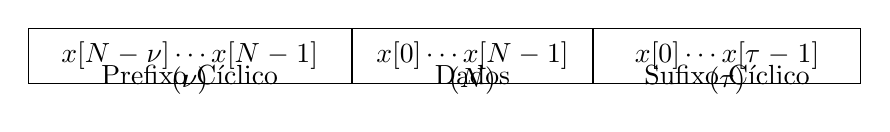
\begin{tikzpicture}[node distance = 2cm, auto]
\node [CE] (Lcp) [xshift=-16.22em] {$x[N-\nu]  \cdots x[N-1]$};
\node [Info] (N) [xshift=-6em] {$x[0] \cdots x[N-1]$};
\node [GI2] (Lcs) [xshift=3.2em] {$x[0]  \cdots x[\tau -1]$};
\node (Lcp_l) [below of=Lcp,yshift=5em] {Prefixo Cíclico} ;
\node (N_l) [below of=N,yshift=5em] {Dados};
\node (Lcs_l) [below of=Lcs,yshift=5em] {Sufixo Cíclico};
\node (Lcp_2) [below of=Lcp_l,yshift=5.5em] {($\nu$)} ;
\node (N_2) [below of=N_l,yshift=5.5em] {($N$)};
\node (Lcs_2) [below of=Lcs_l,yshift=5.5em] {($\tau$)};
\end{tikzpicture}
\caption{Estrutura do símbolo ciclicamente estendido.
\label{fig:structure_ce} }
\end{figure}

Considerando a transmissão de símbolos ciclicamente estendidos, cuja estrutura está apresentada novamente na Figura~\ref{fig:structure_ce}, modela-se o $i$-ésimo símbolo DMT recebido como na Equação~\ref{eq:yideal_yisi_ici}. Esta equação separa o símbolo recebido em três parcelas: o símbolo ideal ($\mathbf{y}_\text{Ideal}$), isto é, o símbolo que resultaria se a convolução linear implementasse perfeitamente uma convolução periódica; o símbolo com valores da ISI no domínio do tempo ($\mathbf{y}_\text{ISI}$) e o símbolo com valores de ICI no domínio do tempo ($\mathbf{y}_\text{ICI}$)
\begin{align}
\mathbf{y}^{(i)}= \mathbf{y}_\text{Ideal}^{(i)} + \mathbf{y}_\text{ISI}^{(i)} + \mathbf{y}_\text{ICI}^{(i)} 
\label{eq:yideal_yisi_ici}
\end{align}

Nota-se que esta representação dos símbolos recebidos é perfeitamente consistente com as definições de ISI e ICI apresentadas. As amostras que estão ausentes no símbolo recebido, as quais impedem que este apresente o resultado de uma convolução periódica, são retiradas pelo vetor $\mathbf{y}_\text{ICI}$ do vetor $\mathbf{y}_\text{Ideal}$. Isto ocorre devido os valores do vetor $\mathbf{y}_\text{ICI}$ corresponderem ao negativo dos elementos de $\mathbf{y}_\text{Ideal}$ que não realidade não estão presentes no símbolo recebido, como mencionado na Seção \ref{sec:ici}. Este conceito ficará claro nas formulações que seguem.

Quando a sincronização simbólica temporal não é considerada, os valores de ISI e ICI são dados através das Equações (2) e (11) em \cite{perodling2002}, respectivamente. Neste caso, o número de amostras do símbolo DMT afetadas por ISI e ICI é dado por $L - \nu$, isto é, a dispersão do canal menos o número de amostras protegidas pelo prefixo cíclico. No entanto, ao considerar a utilização da sincronização e o deslocamento temporal da convolução sob o ponto de vista do receptor, o número de amostras afetadas por ISI e ICI, denominado $N_a$, passa a ser dado por:
\begin{align}
N_a&= L - \nu - n_0
\label{eq:yisi_affected_CE}
\end{align}

Assim, pode-se demonstrar que os valores correspondentes à interferência inter-simbólica no símbolo DMT no domínio do tempo, afetando as primeiras $L - \nu - n_0$ amostras do símbolo, são dados por:	
\begin{align}
y_{ \text{ISI} }^{(i)}[n]  =  \sum \limits_{k = \nu + n_0 + 1 + n }^{ L }      h[k]  x^{(i-1)}[ (( n + \nu + \tau + n_0 -k))_N] \label{eq:yisi_CE_reindexed} \quad \quad \quad 0 \leq n \leq L - \nu - n_0 - 1 
\end{align}
onde $x^{(i-1)}$ é o símbolo DMT no domínio do tempo precedente e o operador $((x))_N$ denota $x$ módulo $N$.

Analogamente, a expressão que determina a ICI no símbolo DMT no domínio do tempo é dada por:
\begin{align}
y_{ \text{ICI} }^{(i)}[n]  &=  -\sum \limits_{k = \nu + n_0 + 1 + n }^{ L }      h[k] x^{(i)}[ ((n +n_0 -k))_N ], \label{eq:yici_CE_reindexed} \quad \quad \quad 0 \leq n \leq L - \nu - n_0 - 1
\end{align}

Ressalta-se na Equação~\ref{eq:yici_CE_reindexed} o sinal negativo antes do somatório, o qual está relacionado com a definição de ICI como a ausência amostras.

\subsection{Representação Matricial}

Alternativamente, pode-se expressar as Equações \ref{eq:yisi_CE_reindexed} e  \ref{eq:yici_CE_reindexed} a partir de matrizes. Neste caso, a Equação~\ref{eq:yideal_yisi_ici} torna-se:
\begin{align}
\mathbf{y}^{(i)} &= \mathbf{y}_\text{Ideal}^{(i)} + \mathbf{y}_\text{ISI}^{(i)} + \mathbf{y}_\text{ICI}^{(i)} \nonumber\\
&= \mathbf{\tilde{H}} \mathbf{x}^{(i)}[ ((n + n_0))_N]  + \mathbf{ H_\text{ISI}} \mathbf{x}^{(i-1)}[ ((n + n_0))_N]  + \mathbf{H_\text{ICI}} \mathbf{x}^{(i)}[ ((n + n_0))_N] 
\nonumber
\end{align}
onde $\mathbf{x}^{(i)}[((n + n_0))_N] $ representa o símbolo DMT no domínio do tempo com deslocamento circular de $n_0$ amostras.

O símbolo recebido ideal é resultado do produto entre a matriz circulante e o símbolo DMT no domínio do tempo com deslocamento circular, já que esta operação equivale à convolução periódica. Portanto,
\begin{align}
\mathbf{y_\text{Ideal}}^{(i)} = \mathbf{ \tilde{H} } \mathbf{x}^{(i)}[((n + n_0))_N] 
\end{align}
onde $\mathbf{ \tilde{H} }$ é a matriz circulante dada na Equação~\ref{eq:circ_h}.

O vetor com o conteúdo de ISI no domínio do tempo é dado pela Equação~\ref{eq:ISI_matrix_rep}, a qual implementa a Equação~\ref{eq:yisi_CE_reindexed} usando a matriz $N \times N$ esparsa de Toeplitz $\mathbf{ H_\text{ISI}}$, definida na Equação~\ref{eq:H_isi_toep}. Isto é:
\begin{align}
\mathbf{y}_\text{ISI}^{(i)} = \mathbf{ H_\text{ISI}} \mathbf{x}^{(i-1)}[((n + n_p))_N] 
\label{eq:ISI_matrix_rep}
\end{align}
onde,
\begin{align}
\mathbf{ H_\text{ISI}} =
\left[
\begin{array}{ccc}
0_{ (L-\nu - n_0) \times \left( N -L + \nu + \tau\right) }  & H_t & 0_{ (L-\nu - n_0) \times \left( n_0 - \tau \right)} \\
\vdots & 0_{ (N - L + \nu + n_0) \times N_a } & \vdots\\
\end{array}
\right]
\label{eq:H_isi_toep}
\end{align}
e $\mathbf{H}_t$ é a matriz de Toeplitz triangular superior, com dimensões $N_a \times N_a$, dada por:
\begin{align}
\mathbf{H}_t
=
\left[
\begin{array}{ccccccc}
h[L] & \cdots &\cdots & \cdots & h[n_0 + \nu +1] \\
0 & h[L] & \cdots &\cdots & h[n_0 + \nu +2]\\
\vdots & & \vdots & \vdots & \vdots \\
0 & 0 & 0 & \cdots & h[L] 
\end{array}
\right]
\label{eq:H_isi_t}
\end{align} 

Similarmente, o vetor com o conteúdo de ICI no domínio do tempo apresentado na Equação~\ref{eq:yici_CE_reindexed} pode ser obtido através da matriz $N \times N$ denominada $\mathbf{ H_\text{ICI}}$, como abaixo:
\begin{align}
\mathbf{y_\text{ICI}}^{(i)} = \mathbf{ H_\text{ICI}} \mathbf{x}^{(i)}[((n + n_p))_N] 
\label{eq:ICI_matrix_rep_vec}
\end{align}
onde
\begin{align}
\mathbf{ H_\text{ICI}} = 
\left[
\begin{array}{ccc}
0_{N_a \times \left( N - L \right) }  & - H_t & 0_{N_a \times \left( \nu + n_0\right) }\\
\vdots & 0_{ N_a\times N_a } & \vdots\\
\end{array}
\right]
\label{eq:H_ici_toep}
\end{align}
